\documentclass{article}
\usepackage{ctex}
\usepackage{float}
\usepackage{geometry}
\usepackage{amsmath}
\usepackage{graphicx}
\geometry{a4paper, scale=0.8}

\title{概率论与数理统计第十一次作业}
\author{ZhaohengLi 2017050025}

\begin{document}
\maketitle

\section{4.4.4}
由题意可以知道:

$$E(X_i)=3.5,\quad Var(X_i)=\frac{35}{12},\quad E(\overline X)=3.5,\quad Var(\overline X)=\frac7{240}$$

根据林德伯格-莱维中心极限定理可以知道:

$$P(3\leq \overline X \leq 4)\approx \Phi (\frac{4-3.5}{\sqrt{7/240}})-\Phi (\frac{3-3.5}{\sqrt{7/240}})=0.9966$$


\section{4.4.9}
设$X_i$为第$i$位顾客的消费额,那么$X_i\sim U(20,100)$,因此$E(X_i)=60,Var(X_i)=\frac{1600}{3}$。

设餐厅的每天营业额为$Y=\sum^{400}_{i=1}X_i$。

(1)
$$E(Y)=\sum^{400}_{i=1}E(X_i)=24000$$

(2)
根据林德伯格-莱维中心极限定理可以知道:

$$P(-760<Y-2000<760)\approx 2\Phi(\frac{760}{\sqrt{400*1600/3}})-1=0.9$$
\section{4.4.19}

设:

\begin{equation}
X_i = \left\{
\begin{aligned}
&1,& room\quad i\quad is\quad taken,\\
&0,& room\quad i\quad is\quad not\quad taken.\\
\end{aligned}
\right.
\end{equation}

因此有$X_i\sim b(1,0.8),Y=X_1+X_2+\dots+X_{500}\sim b(500,0.8)$。

$$P(2Y\leq k)=P(Y\leq \frac k2)\geq 0.99$$
$$\Phi(\frac{k/2+0.5-500*0.8}{\sqrt{500*0.8*0.2}})\geq 0.99$$

因此,查表可知,$k>840.68$,即每天需要841千瓦电力才能满足要求。


\section{4.4.26}
$$E(Y_n)=\frac 1n\sum^n_{i=1}E(X^2_i)=\alpha_2$$
$$Var(Y_n)=\frac1{n^2}\sum^n_{i=1}Var(X_i^2)=\frac{\alpha_4-\alpha^2_2}{n}$$

% \section{5.2.3}
% 首先求出组距:

% $$d=\frac{1572-736}{6}\approx 140$$

% 频率分布表为:

% \begin{table}[H]
% \centering
% \begin{tabular}{|c|c|c|c|c|c|}
% \hline
% 组序 & 区间            & 中值   & 频数 & 频率   & 累计频率 \\ \hline
% 1  & (735,875{]}   & 805  & 6  & 0.20 & 0.2  \\ \hline
% 2  & (875,1015{]}  & 945  & 8  & 0.27 & 0.47 \\ \hline
% 3  & (1015,1155{]} & 1085 & 9  & 0.30 & 0.77 \\ \hline
% 4  & (1155,1295{]} & 1225 & 4  & 0.13 & 0.90 \\ \hline
% 5  & (1295,1435{]} & 1365 & 2  & 0.07 & 0.97 \\ \hline
% 6  & (1435,1575{]} & 1505 & 1  & 0.03 & 1.00 \\ \hline
% 合计  & &  & 30 & 1 & \\ \hline
% \end{tabular}
% \end{table}

% 直方图为:

% \begin{figure}[H]
%     \centering
%     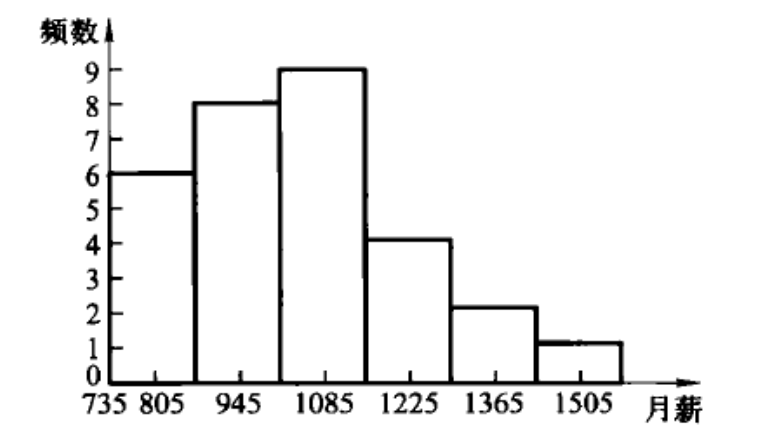
\includegraphics[width=0.5\textwidth]{pic1.png}
%     \caption{}
% \end{figure}

% \section{5.2.5}
% 首先求出组数:

% $$k=\frac{14667-353}{1700}=8.42$$

% 因此分9组。

% 之后求出端点:

% $$a_0<353,\quad a_0+9*1700>14667$$

% 取$a_0=300$。

% 频率分布表为:

% \begin{table}[H]
% \centering
% \begin{tabular}{|c|c|c|c|c|c|}
% \hline
% 组序 & 区间            & 中值   & 频数 & 频率   & 累计频率 \\ \hline
% 1  & (300,2000{]}   & 1150  & 12  & 0.3 & 0.3  \\ \hline
% 2  & (2000,3700{]}  & 2850  & 6  & 0.15 & 0.45 \\ \hline
% 3  & (3700,5400{]} & 4550 & 5  & 0.125 & 0.575 \\ \hline
% 4  & (5400,7100{]} & 6250 & 6  & 0.15 & 0.725 \\ \hline
% 5  & (7100,8800{]} & 7950 & 3  & 0.075 & 0.8 \\ \hline
% 6  & (8800,10500{]} & 9650 & 0  & 0 & 0.8 \\ \hline
% 7  & (10500,12200{]} & 11350 & 1  & 0.025 & 0.825 \\ \hline
% 8  & (12200,13900{]} & 13050 & 4  & 0.1 & 0.925 \\ \hline
% 9  & (13900,15600{]} & 14750 & 3  & 0.075 & 1 \\ \hline
% 合计  & &  & 40 & 1 & \\ \hline
% \end{tabular}
% \end{table}


% 直方图为:

% \begin{figure}[H]
%     \centering
%     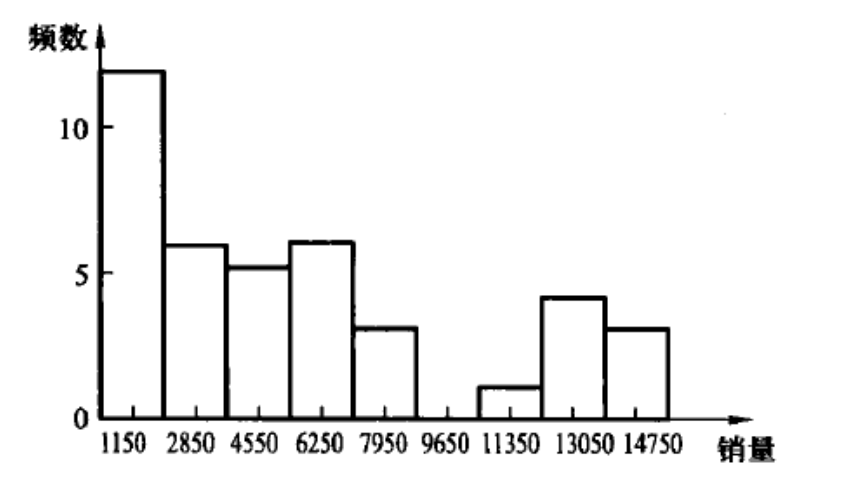
\includegraphics[width=0.5\textwidth]{pic2.png}
%     \caption{}
% \end{figure}

\section{5.3.3}

$$\overline y=\frac1n\sum^{n}_{i=1}y_i=\frac1n\sum^{n}_{i=1}(3x_i-4)=3\overline x -4$$

$$s^2_y=\frac{1}{n-1}\sum^{n}_{i=1}(y_i-\overline y)^2=\frac{1}{n-1}\sum^{n}_{i=1}9(x_i-\overline x)^2=9s_x^2$$
\section{5.3.5}

因为:
$$\overline x_1 = \frac{x_{11}+x_{12}+\cdots+x_{1n}}{n},\overline x_2=\frac{x_{21}+x_{22}+\cdots+x_{2m}}{m}$$

所以:

$$\overline x = \frac{x_{11}+x_{12}+\cdots+x_{1n}+x_{21}+x_{22}+\cdots+x_{2m}}{n+m}=\frac{n\overline x_1+ \overline x_2}{n+m}$$

因为:

$$s_1^2=\frac1{n-1}\sum^n_{i=1}(x_{1i}-\overline x_1)^2,s_2^2=\frac1{m-1}\sum^m_{i=1}(x_{2i}-\overline x_2)^2$$

所以:

$$s^2=\frac{1}{n+m-1}[\sum^n_{i=1}(x_{1i}-\overline x)^2+\sum^m_{i=1}(x_{2i}-\overline x)^2]$$
$$=\frac{(n-1)s_1^2+(m-1)s_2^2}{n+m-1}+\frac{n(\overline x_1-\frac{n\overline x_1+m\overline x_2}{n+m})^2+m(\overline x_2-\frac{n\overline x_1+m\overline x_2}{n+m})^2}{n+m-1}$$
$$=\frac{(n-1)s_1^2+(m-1)s_2^2}{n+m-1}+\frac{nm(\overline x_1 - \overline x_2)^2}{(n+m)(n+m-1)}$$

\section{5.3.9}
设总体方差为$\sigma^2$,那么有:

$$Corr(x_i-\overline x,x_j-\overline x)=\frac{Cov(x_i-\overline x, x_j-\overline x)}{\sqrt{Var(x_i-\overline x)}\sqrt{Var(x_j-\overline x)}}$$

$$Cov(x_i-\overline x, x_j-\overline x)=-\frac{\sigma^2}{n}$$
$$Var(x_i-\overline x)=Var(x_j - \overline x)=Var(x_1 - \overline x)=\frac{(n-1)\sigma^2}{n}$$

$$Corr(x_i-\overline x,x_j-\overline x)=-(n-1)^{-1}$$

\section{5.3.10}


$$\sum_{i<j}(x_i-x_j)^2=(n-1)\sum^n_{i=1}x^2_i-2\sum_{i<j}x_ix_j$$

$$(\sum^n_{i=1})^2=\sum^n_{i=1}x^2_i+2\sum_{i<j}x_ix_j$$

因此有:

$$\sum_{i<j}(x_i-x_j)^2=n\sum^n_{i=1}x_i^2-(\sum^n_{i=1}x_i)^2=n\sum^n_{i=1}(x_i-\overline x)^2$$


\section{5.3.23}

首先可以得到:
$$P(x_{(n)}\leq k)=P(x_1\leq k,\cdots,x_n\leq k)=(1-q^{k})^n, k=1,2,\cdots$$

$$P(x_{(n)}\leq k-1)=(1-q^{k-1})^n, k=1,2,\cdots$$


$$P(x_{(n)}\leq 0)=0$$
$$P(x_{(n)}= k)=(1-q^{k})^n-(1-q^{k-1})^n, k=1,2,\cdots$$

其满足非负性和正则性。

$$\sum^{+\infty}_{k=1}P(x_{(n)}=k)=lim_{m\rightarrow +\infty}\sum^m_{k=1}[(1-q^k)^n-(1-q^{k-1})^n]=lim_{m\rightarrow +\infty}(1-q^m)^n=1$$


$$P(x_{(1)}\geq k)=(P(x_1\geq k))^n=q^{n(k-1)}, k=1,2,\cdots$$
$$P(x_{(1)}\geq k+1)=q^{nk}, k=1,2,\cdots$$

最终求得分布列为:

$$P(x_{(1)=k}=P(x_{(1)}\geq k)-P(x_{(1)}\geq k+1)=q^{n(k-1)}(1-q^n), k=1,2,\cdots$$

经验证,上述分布列满足非负性和正则性。

\section{5.3.24}
(1)

$$P(x_{(16)}>10)=1-P(x_{(16)}\leq10)=1-(P(x_1\leq 10))^{16}=0.937$$

(2)

$$P(x_{(1)}>5)=(P(x_i>5))^{16}=(1-\Phi(\frac{5-8}2))^{16}=0.3308$$

\end{document}





